\chapterimage{/5/head.jpg} % Chapter heading image
\chapter{Storia Cronologica dell'Universo}\label{5:ch}

Non ci si avventurerà nella selva oscura della teoria GUT, ma verranno soltanto citati graficamente i fenomini-chiave e i principali periodi che caratterizzano le primissime fasi di vita del nostro universo. A partire dal tempo di Plank, $t_P=10^{-43}$ s, gli effetti quantistici diminuiscono col passare degli istanti, ma leptoni e adroni sono ancora la stessa cosa. Per questo motivo in questa fase può essere violata la conservazione del numero barionico ($n_b + n_{\overbar{b}}$). Possono cioè verificarsi reazioni che ristabiliscano l'equilibrio in seguito a qualsivoglia deviazione da esso: $n_b = n_{\overbar{b}}$. La transizione GUT è l'unico momento in cui può essersi formata l'anisotropia di 1 parte su $10^8$ barioni (i modelli di bariogenesi faticano ancora a trovare un valore così piccolo). Inoltre in questi istanti si formano le cariche, tra cui i monopoli magnetici. Durante la fase intermedia successiva, che dura $10^{-26}$ secondi, la temperatura cala di $12$ dex e alla fine si ha $R_H = 1$ cm. La fisica delle particelle fatica a trovare candidati per questo range di temperature, per questo il periodo viene definito \textit{deserto di particelle}. La seconda transizione importante è quella elettrodebole, durante la quale i leptoni e il neutrino possono prendere massa. Infine all'ultima transizione quark-adroni si ha $R_H = 1$ km. 

\begin{figure}[H]
    \centering
    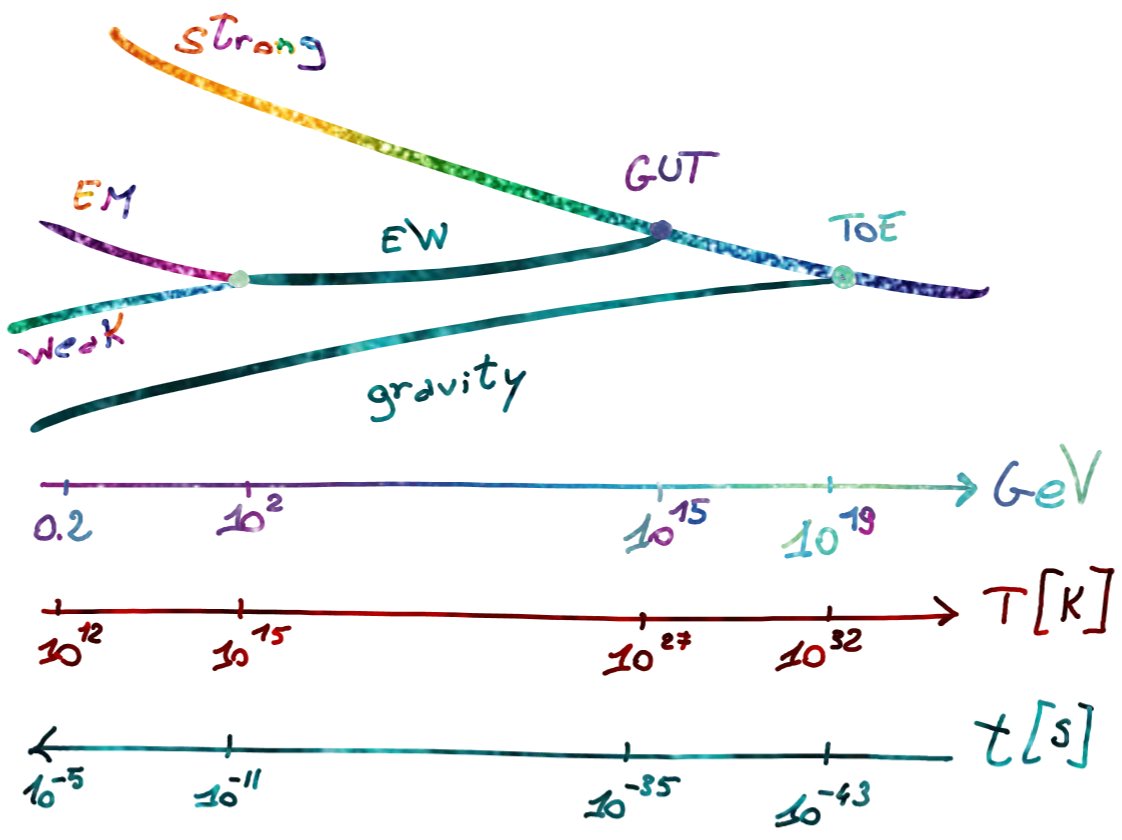
\includegraphics[width=.75 \textwidth]{Pictures/5/fasiprimordiali.png}
    \label{fig:4}
\end{figure}


\section{Modello di Guth (\textit{old inflation})}
I primo modelli di inflazione (anni `80) si basavano sulla teoria delle transizioni di fase del primo tipo. La temperatura critica precedentemente definita, è in questo caso la temperatura della transizione GUT e $\phi$ viene chiamato \textbf{inflatone}. A $T=T_{GUT}$ si iniziano a sviluppare due nuovi minimi allo stesso livello del vecchio e si viene quindi a creare una posizione di falso equilibrio o \textit{falso vuoto}. Al calare della temperatura il sistema non raggiunge istantaneamente la posizione di equilibrio a causa della barriera di potenziale dovuta alla forma di $\phi$. Quando la barriera di potenziale viene vinta il sistema è sovra-raffreddato e, raggiungendo il nuovo equilibrio, libera il calore latente (\textbf{reheating}). È quest'ultimo processo che può spiegare la generazione e termalizzazione di un grande numero di particelle.

La densità di lagrangiana dell'inflatone è: $\mathcal{L}_\phi = 1/2 \dt{\phi}^2-V(\phi, T)$ dove $V(\phi, T)$ è il potenziale che corrisponde al campo scalare dell'inflatone e fa il gioco dell'energia libera. Il contributo dell'inflatone al tensore energia-impulso vale:
\begin{equation*}
    T \phi_{ij}=-p_\phi g_{ij}+(p_\phi -\rho_\phi)~u_i u_j \qquad \left\{
        \def\arraystretch{1.5}
            \begin{array}{ll}
                p_\phi = \mathcal{L}_\phi = \frac{1}{2}\dt{\phi}^2-V \\
                \rho_\phi = \frac{1}{2}\dt{\phi}^2+V 
        \end{array}\right.
\end{equation*}
Dall'equazione di Eulero-Lagrange si trova l'\textit{equazione fondamentale della dinamica dell'inflatone}:
\begin{equation}
    \ddt{\phi} + 3H \dt{\phi} + \frac{\partial V}{\partial \phi} =0
\end{equation}
in cui $3H\dt{\phi}$ gioca il ruolo di termine di frizione. Il ``moto'' dovrà essere rallentato affinché l'inflazione duri a sufficienza. Includendo questi contributi nelle equazioni di Friedmann (ponendo $c=1$), si può verificare che l'espansione risultante è accelerata:
\begin{equation*}
\left( \frac{\dt{a}}{a}\right)^2 = \frac{8\pi}{3}G\rho_\phi \qquad \rho_\phi \simeq V \qquad \rightarrow \qquad a=a_0 ~e^{t/\tau} \qquad \tau^{-1} = \sqrt{8\pi G V /3}
\end{equation*}
Inoltre, assumendo un valore del potenziale $V$ si può calcolare il numero di e-folding:
\begin{equation*}
N_{ef} = -8\pi G \int_{\phi_i}^{\phi_f} \left(\frac{\mathrm{d} \ln V}{\mathrm{d}\phi}\right)^{-1}\mathrm{d}\phi
\end{equation*}
che cresce, ovviamente, quanto più è piatto il potenziale. 

Il problema di questi modelli è che prevedono una dimensione di $R_H$ insufficiente per coprire l'intero universo, si creano delle ``bolle di universo'' troppo piccole. Si è quindi passati a considerare le transizioni del secondo tipo, nonostante non offrano le possibilità di un rilascio di energia sotto forma di calore latente. Queste transizioni prevedono un inizio istantaneo dell'inflazione, quindi la forma del potenziale dovrà essere regolata in modo tale che l'inflazione duri a sufficienza. Anche tali \textbf{new inflation models} non sono stati apprezzati perché richiedono un \textit{fine-tuning} dei parametri.

\section{Modello di inflazione caotica}
Il paradigma attuale dell'inflazione, l'inflazione caotica, è dovuto a Linde e non si basa sulle transizioni di fase. È sufficiente che esista un campo scalare estremamente energetico e statico nella fase iniziale, $\phi$. L'equazione della dinamica, la densità e la pressione dell'inflatone sono le stesse.
\subsection{Potenziale quadratico}
Per semplificare i conti si utilizzano le unità planckiane (\ref{eq:unitaplanckiane}) e si assume un potenziale della forma:
$$
V(\phi)= \frac{m^2~\phi^2}{2}
$$
dove $m$ è la massa dello scalare corrispondente all'inflatone. L'equazione della dinamica dell'inflatone diventa:
\begin{equation}
    \ddt{\phi} + \sqrt{12 \pi} \left( \dt{\phi}^2+m^2 \phi^2 \right) \dt{\phi} + \frac{\partial V}{\partial \phi} =0
\end{equation}

Questa può essere studiata nello spazio delle fasi ($\phi, \dt{\phi}$) ed essendo del II ordine non autonoma vale la relazione $\ddt{\phi} = \dt{\phi} ~ \mathrm{d} \dt{\phi} /\mathrm{d} \phi$. Partendo con la condizione in cui il termine cinetico domina su quello potenziale, la traiettoria può essere studiata in tre fasi principali: caduta sull'attrattore, inflazione e graceful exit (Fig. \ref{fig5:chaotic}).

\vspace{1em}
\begin{example}[Caduta sull'attrattore] $\dt{\phi}^2 \gg m^2 \phi^2 \qquad p_\phi = \rho_\phi = \frac{\dt{\phi}}{2} \rightarrow w=1$ (\textit{ultra hard equation of state})
\end{example}
\noindent A differenza dei modelli visti in precedenza non è richiesto un particolare \textit{fine-tuning} dei parametri, ma si parte da generici valori iniziali $\dt{\phi} \gg \phi$. Dall'equazione della dinamica modificata si può ottenere l'andamento delle traiettorie in questo primo regime:
\begin{equation}
    -\dt{\phi} \frac{\mathrm{d} \dt{\phi}}{\mathrm{d} \phi} = \sqrt{12 \pi} \dt{\phi}^2 \quad \rightarrow \quad \dt{\phi} \propto e^{\sqrt{12 \pi} \phi}
\end{equation}
Integrandole in funzione del parametro tempo $t$:
\begin{equation}
    \phi= cost - \frac{\ln t}{\sqrt{12 \pi}} \qquad \dt{\phi} = \frac{1}{\sqrt{12 \pi}}\frac{1}{t};
\end{equation}
da cui è chiaro che in questa fase la traiettoria è praticamente parallela all'asse $\dt{\phi}$ ($\delta \phi \ll \delta\dt{\phi}$ ). Dalle equazioni di Friedmann si può inoltre verificare che l'andamento dei principali parametri cosmogici è lo stesso di un universo EdS con $w=1$:
\begin{equation}
    H = \frac{1}{3t} \qquad a \propto t^{1/3} \qquad \rho \propto a^{-6}
\end{equation}

In conclusione, se il campo scalare parte con un'energetica sufficiente, il sistema raggiunge naturalmente un $\phi$ poco differente dal valore iniziale a seguito di una forte diminuzione di $\dt{\phi}$.

\vspace{1em}
\begin{example}[Inflazione] 
    $\mathrm{d} \dt{\phi} / \mathrm{d} \phi=0 \qquad m\phi_i \gg \dt{\phi}_i$
\end{example}

Queste due assunzioni sono finalizzate al risultato finale, ossia quello di avere una fase inflazionaria sufficientemente lenta, in particolare è richiesto che il valore di inserzione $\phi_i$ sul cosiddetto \textbf{attrattore} sia sufficientemente alto. 
\begin{equation}
    \dt{\phi} =  -\frac{m}{\sqrt{12 \pi}} = cost \qquad \phi= \phi_i - \frac{m}{\sqrt{12 \pi}} (t-t_i) = \phi_f - \frac{m}{\sqrt{12 \pi}} (t-t_f); \label{eq:phidotphiinfl}
\end{equation}

Si assume $\phi_f = 0$, per cui il valore del potenziale sull'attrattore è $V= m^4 (t_f-t)^2 / 24 \pi$. L'inflazione termina quando $\ddt{a}=0$, ossia $\rho_\phi = -3p_\phi = m^2 / 8 \pi$. Dato che in questo regime $\rho_\phi \approx V$ si ha:
$$
\phi_f = \sqrt{\frac{1}{4\pi}}= \mathcal{O}(1)
$$
Il potenziale alla fine di questa fase è quindi dell'ordine di 1 volta il potenziale al tempo di Planck. Dalle equazioni di Friedmann si può inoltre calcolare l'andamento dei principali parametri cosmogici:
\begin{equation}
    H^2 = \frac{8\pi }{3}\rho_\phi \rightarrow H = \frac{m^2}{3} (t_f -t) \qquad a=a_f e^{-m^2 (t_f-t)^2 /6} \qquad a=a_i e^{(H+H_i)(t-t_i)^2 /2}
\end{equation}
Si nota che $H$ descresce in modo lineare nel tempo, mentre $a$ si espande in modo esponenziale: \textbf{inflazione}. Per risolvere i problemi dell'età dell'universo e dell'orizzonte si applica la condizione $\ln (a_f/a_i) \gg 60$ assumendo $\phi_f = 0$ e utilizzando l'equazione (\ref{eq:phidotphiinfl}):
\begin{equation}
    2 \pi \phi_i^2 \gg 60 \quad \rightarrow \quad \phi_i \gg 3 \div 4
\end{equation}
Questo significa avere valori di $\phi$ più grandi di quelli al tempo di Planck, ma la fisica è dettata da $V$. La condizione per non dover includere anche effetti quantistici è $V_i<1$, ossia: $m^2 \phi_i^2 /2 <1$. A $m=m_{GUT}$ si deve avere $\phi_i < 10^4$ unità plankiane: la condizione su $\phi_i$ può quindi essere valida.

\vspace{1em}
\begin{example}[Graceful Exit] 
    $H^2=\frac{4\pi }{ 3} \left(\dt{\phi}^2 +m^2\phi^2\right) \qquad \ddt{\phi} + 3H \dt{\phi} + \frac{\partial V}{\partial \phi} =0$
\end{example}
In questa fase si utilizzano tutti i termini dell'equazione della dinamica. Dalla prima equazione: 
\begin{equation}
    \dt{\phi} \equiv \sqrt{\frac{3}{4\pi}} ~H \sin \theta, \quad m\phi \equiv \sqrt{\frac{3}{4\pi }} ~H \cos \theta
\end{equation}
dove $\theta$ rappresenta l'angolo che descrive la traiettoria nello spazio ($\dt{\phi}, m\phi$). Derivando temporalmente le quantità $(H\sin\theta)$ e $(H\cos\theta)$ si ottengono le relazioni:
\begin{equation}
    \dt{H} = -3H^2 \sin^2 \theta \qquad\qquad  \dt{\theta} \propto -m \qquad \theta \propto -mt
\end{equation}
La derivata del parametro di Hubble oscilla nel tempo, ma è smorzata all'aumentare di H e l'angolo di fase varia linearmente. Integrando nel tempo si può ottenere il valore di $H$ e $a$ per $mt$ piccoli:
\begin{equation}
    H = \frac{2}{3t}\left( 1+ \mathrm{sinc} (2mt)\right) + \mathcal{O}(t^{-3}) \qquad\qquad a\propto t^{2/3}
\end{equation}
La $\mathrm{sinc}$ smorza l'ampiezza della spirale di H. Questo risultato non ci soddisfa particolarmente, perché usciremmo dall'inflazione con un'equazione di stato che non corrisponde alla componenete radiativa ($a_{EdS}\propto t^{1/2}$). Lo smorzamento sarà comunque il meccanismo che genererà le fluttuazioni di inflatone (particelle).


\begin{figure}[H]
    \centering
    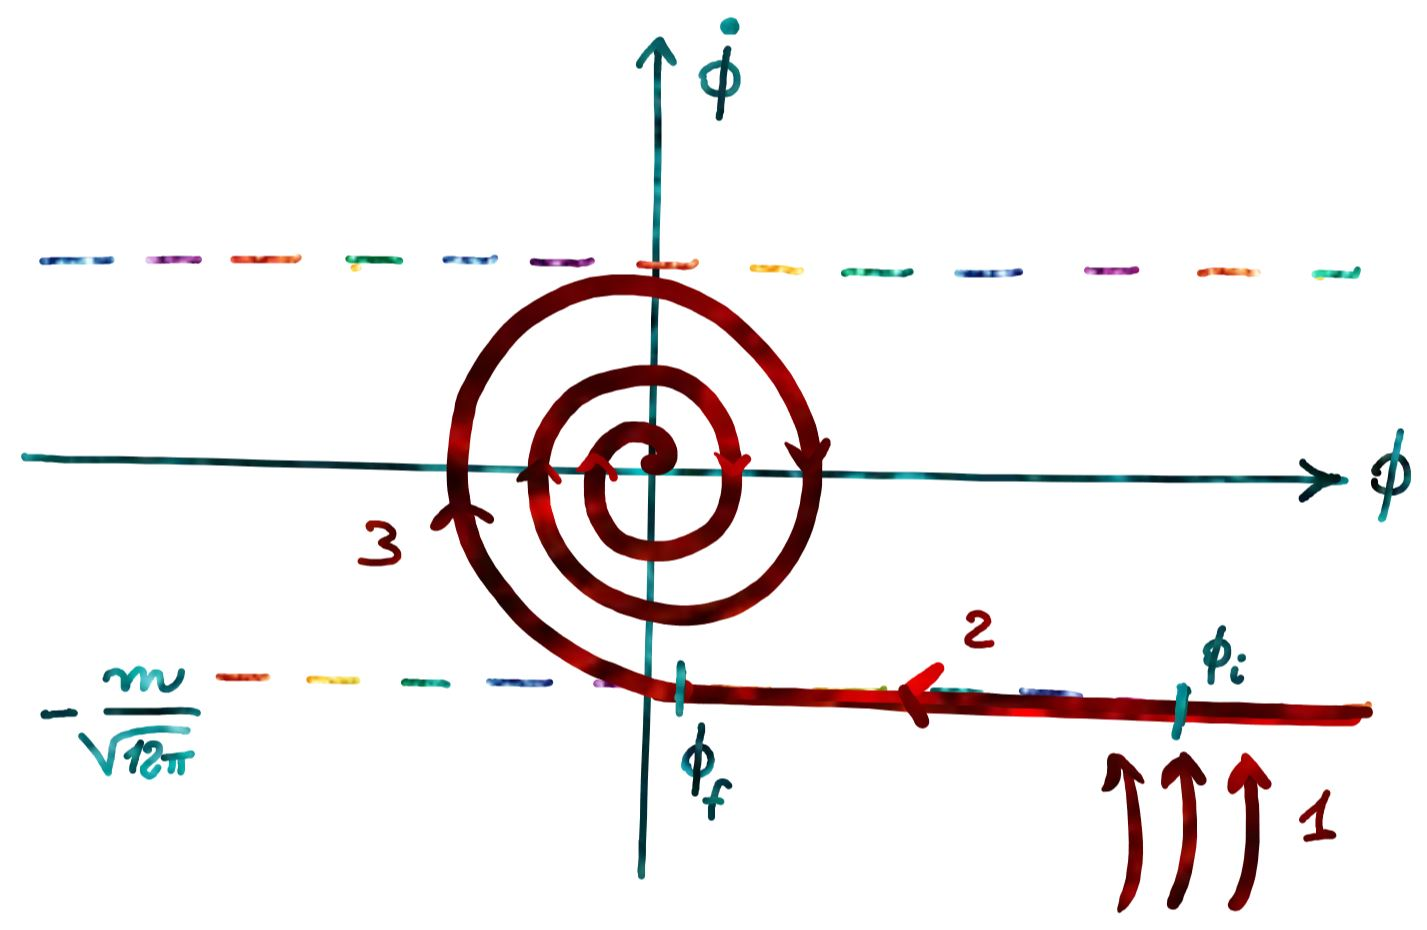
\includegraphics[width=.9 \textwidth]{Pictures/5/chaosinfl.jpg}
    \caption{Diagramma di fase per il modello di inflazione caotica. Si distinguono le tre fasi principali: (1) caduta sull'attrattore, (2) inflazione, (3) graceful exit. Per il potenziale quadratico si ha: $\phi_i\gg  4$ e $\phi_f = \mathcal{O} (1)$. Comportamenti speculari si avrebbero partendo dal secondo quadrante.}\label{fig5:chaotic}
\end{figure}


\subsection{Potenziali generalizzati}\label{ch5:epsieta}
Per forme del potenziale diverse da quella quadratica (bocciata dal satellite Plank) valgono comunque le equazioni:
\begin{equation*}\left\{
    \def\arraystretch{1.5}
        \begin{array}{ll}
            \ddt{\phi} + 3H \dt{\phi} + \frac{\partial V}{\partial \phi} =0\\ 
            H^2 = \frac{8\pi}{3} \left(\dt{\phi}^2+V\right)
    \end{array}\right.
\end{equation*}

Per risolvere i problemi dell'orizzonte e della piattezza si introducono le condizioni di lento rotolamento (\textbf{slow roll}):
\begin{equation}
    \left| \dt{\phi}^2 \right| \ll \left| V \right|  \qquad\qquad \left| \ddt{\phi} \right| \ll \left| 3H\dt{\phi} \right|;
\end{equation}
che corrispondono rispettivamente alle richieste che il termine potenziale sia dominante rispetto a quello cinetico e l'accelerazione domini sul termine di frizione. In questo modo si ottiene $a'/a = -8\pi V/V'$ (l'apice indica la derivata rispetto a $\phi$), da cui:
\begin{equation}
    60 \ll N_{ef} = 8\pi \int_\phi^{\phi_i} \frac{V}{V'} \mathrm{d}\phi. 
\end{equation}
In letteratura le condizioni di slow rolling vengono riscritte sotto forma di $V'$ e $V''$:
\begin{equation}
    \left| \left( V'/V\right)^2 \right| \ll 1 \qquad\qquad \left|  V''/V \right| \ll 1;
\end{equation}
e vengono introdotti i seguenti parametri:
\begin{equation}
    \varepsilon = \frac{1}{16\pi}\left(\frac{V'}{V}\right)^2 \qquad\qquad \eta = \frac{1}{8\pi}\left|\frac{V''}{V}\right|
\end{equation}
In generale bisogna avere $\varepsilon, \eta \ll 1$ (in unità planckiane), ma i valori precisi vengono calcolati per ogni nuovo modello, perché lasciano caratteristiche osservabili sulla CMB e nella struttura a larga scala (deviazioni dalla perfetta gaussianità). In pratica l'inflazione è falsificabile attraverso questi due numeretti. Un potenziale a legge di potenza $V=\lambda \phi^n / n$ ha le seguenti caratteristiche:
\begin{equation}
    \varepsilon =   \frac{1}{16\pi} \left( \frac{n}{\phi}\right)^2 \qquad \eta= 2 \frac{n-1}{n} ~\varepsilon \qquad\qquad a(\phi)=a_i ~e^{N_{ef}} = a_i ~e^{4\pi(\phi_i^2-\phi)/n}
\end{equation}
ossia restituisce sempre un'espansione esponenziale che può essere regolata tramite $n$ per ottenere l'$N_{ef}$ desiderato.

\subsection{Reheating}
La termalizzazione è possibile grazie all'elevata quantità di energia disponibile e può essere legata al decadimento dell'inflatone. Questo processo può avvenire in due modi:
$$
\phi \rightarrow \chi + \chi \qquad \phi \rightarrow \psi + {\overbar{\psi}}
$$
nel primo caso viene prodotta una coppia di scalari e nel secondo una coppia fermione-antifermione. La lagrangiana di interazione è $\Delta \mathcal{L} = -g \phi \chi^2 - h \phi \psi {\overbar{\psi}}$ dove $g$ e $h$ sono le costanti di accoppiamento dei due processi. I rispettivi tassi di decadimento sono dati dalle seguenti relazioni:
$$
\Gamma_\chi = g^2 / 8\pi m \qquad \Gamma =h^2 m / 8\pi 
$$
Per evitare di entrare nel regime quantistico bisogna che $g \lesssim m$ e $h\lesssim m^{1/2}$, quindi si possono assumere $\Gamma_\chi \approx m$ e $\Gamma_\psi \approx m^2$. Per cui a $m_{GUT}=10^{-4}$ si ha $\Gamma_\psi \ll \Gamma_\chi$ e domina il processo di decadimento degli scalari. La variazione di densità numerica degli scalari seguirà quindi la legge: $\dt{n}_\phi = - g^2 ~n_\phi / 8\pi m$. Il numero di oscillazioni dello scalare inflatone nell'unità di tempo (``giri di spirale'') è: $N_{osc}=mt/2\pi$, per cui passando per il differenziale $\mathrm{d}n_\phi$ si ha:
\begin{equation}
    n_\phi \propto e^{-g^2 ~N_{osc}/4m^2}
\end{equation}
Sostituendo $g \sim m$ sono sufficienti pochissime oscillazioni per far decadere tutti gli inflatoni e formare gli scalari $\chi$. Anche per $g \ll m$ questo è verificato, grazie al contributo di processi di risonanza e condensazioni di Bose. Inoltre, assumendo che la massa dell'inflatone sia $m=10^{13}$ GeV ($10^{-6}$ unità planckiane):
\begin{equation}
    n_\phi (t_f)\approx \frac{1}{2}m\phi_f^2 \approx 10^{92}\; \mathrm{cm^{-3}}
\end{equation}
si ottengono un sacco di particelle e tutta l'entropia che potrebbe servire. Oggi l'energia dell'universo è talmente bassa che processi come questo non possono avere luogo, l'inflazione va collocata a livelli energetici alti.

\subsubsection{Temperatura di Reheating}
La temperatura in uscita del processo di inflazione deve necessariamente essere $T_{RH}<T_{GUT}\simeq 10^{16}$ GeV, altrimenti si riattraverserebbe ciclicamente la transizione GUT (pb. monopoli magnetici e cose di questo tipo). In ogni caso è necessario termalizzare l'universo, ossia $\Gamma_\chi^{-1}<H^{-1}$, nel limite in cui si equivalgono (corrispondente alla fine del processo) si ha:
\begin{equation}
    \Gamma_\chi \simeq \frac{m}{8\pi} \quad\equiv\quad H \simeq \sqrt{\frac{8\pi^3}{90}g^* T^4}\quad \rightarrow \quad T_{RH} = 2\cdot 10^{-4} \left( g^*_{100} \right)^{-1/2} \left( m_{\phi, -6} \right)^{1/2}
\end{equation}
La cosiddetta temperatura di reheating dipende quindi dalla massa dell'inflatone, nel caso in cui $m_\phi = 10^{-6}$ si avrebbe $T_{RH}\approx 10^{-4}\;\mathrm{T_P}=10^{15}$ GeV che è già pericoloso! 

\newpage
\subsubsection{Sommario}
Il paradigma dell'inflazione si aggiunge al modello del Big Bang per risolvere tre dei cinque problemi: orizzonte, piattezza e monipoli magnetici. Il problema dell'orizzonte si ha perché vediamo la connessione causale su regioni dell'universo che sono più grandi della regione dell'orizzonte e viene risolto assumendo che la connessione causale era stata raggiunta già prima. Il problema della piattezza si riferisce a una richiesta di perfetto bilanciamento tra energia cinetica e potenziale. Inoltre il modello del Big Bang prevederebbe oggi un'alta densità di monopoli magnetici che avrebbero dovuto chiudere immediatamente l'universo e comunque non sono stati osservati. I primi due problemi possono essere risolti mediante un'espansione accelerata dell'universo che inverte i comportamenti del raggio dell'orizzonte e del parametro di densità totale. La durata di questa espansione deve comunque essere sufficientemente lunga: la condizione richiesta dal primo problema $N_{ef} \gg 60$, soddisfa pienamente anche il secondo. 

Storicamente i primi modelli si sono appoggiati alle transizioni di fase perché avvengono all'energetica richiesta e generano le particelle desiderate. La dinamica è descritta dall'equazione fondamentale dell'inflazione che è derivata dall'equazione di Eulero-Lagrange per l'inflatone (parametro d'ordine delle transizioni di fase). Applicando le condizioni di slow rolling si ottengono: espansione accelerata e un numero sufficiente di e-folding. In particolare i modelli old inflation utilizzavano le transizioni del primo tipo, mentre quelli new inflation le transizioni del secondo tipo. Si è poi concluso che non funzionavano perché non riuscivano a generare regioni abbastanza grandi da contenere il nostro universo e richiedevano un fine-tuning dei parametri.

Il modello attuale è quello dell'inflazione caotica. La dinamica dell'inflatone, ora inteso come campo scalare estremamente energetico, è descritta dalla stessa equazione di cui sopra. In questo caso si può avere un ampio range di condizioni iniziali che generano quasi tutte la stessa traiettoria, infatti inizialmente le curve cadono sull'attrattore e da qui ha inizio l'inflazione (non è più richiesto un fine-tuning). Durante la fase di inflazione, $\phi_i \rightarrow \mathcal{O}(1)$, si ha espansione accelerata e si può avere l'$N_{ef}$ necessario purché $\phi_i \gg 3\div 4$. Inoltre la richiesta di non entrare in regime quantistico $V<1$ si traduce in un limite superiore a $\phi_i$. In conclusione, $ 3 \ll \phi_i < 10^4$ in unità planckiane. In questo modo si può stabilire quale valore (naturalmente al di sotto di $m_P$) associare alla massa dello scalare inflatone, e.g. $m_\phi = 10^{-6}$. Si può dimostrare che questo approccio vale anche per forme del potenziale $V$ leggermente diverse da quella quadradica. 

Quando si esce dalla fase di inflazione, $\phi = \mathcal{O}(1)$, si può innestare un meccanismo di decadimento dello scalare inflatone. La fisica delle particelle garantisce che il processo dominante è quello di decadimento in due scalari e anche pochi giri di spirale sono sufficienti per riempire l'universo di particelle. Inoltre, per avere $w=1/3$ in uscita, si può termalizzare l'universo purché la temperatura di reheating rimanga minore della temperatura GUT. Lo ``stiramento'' provocato dall'inflazione appiattisce l'universo e qualunque perturbazione ci sia in esso, all'uscita quindi l'universo è omogeneo e isotropo (\textit{cosmic no hair theorem}).

\vspace{1em}
\noindent Alcune predizioni dell'inflazione sono falsificabili: 
\begin{itemize}
    \item[-] $\Omega_{TOT} = 1$, universo piatto (confermato da Planck a meno di $10^{-2}$);
    \item[-] Le particelle generate creano fluttuazioni pressoché gaussiane nel campo di densità;
    \item[-] Distribuzione della scala angolare del campo di densità (pressoché \textit{scale invariant});
    \item[-] Piccole deviazioni da gaussianità e invarianza di scala legate a $\varepsilon \leftrightarrow  V' $ e $\eta \leftrightarrow V''$;
    \item[-] Fluttuazioni tensoriali (onde gravitazionali).
\end{itemize}

\vspace{1em}
In conclusione, l'inflazione non è un modello, è un paradigma, una famiglia di modelli che hanno in comune la richiesta di avere campi sufficientemente energetici. Si distinguono dall'avere predizioni diverse per $\varepsilon$, $\eta$ e onde gravitazionali. Con i dati di Plank una buona serie di modelli inflazionari è stata rigettata, ma ci sono ancora più modelli che teorici al mondo. Il vantaggio di studiare la CMB piuttosto che la LSS sta nel fatto che ha molta più memoria (perché è più temporalmente vicina) delle condizioni iniziali. 


\section{L’era adronica e l’era leptonica}
L'ultima delle grandi transizioni di fase, la transizione quark-adroni, avviene a $T=200\div 300$ MeV a circa $10^{-5}$ s. Da questo istante i quark si possono unire per dare origine agli adroni. 

\subsection{Era adronica}
Le reazioni che caratterizzano questo periodo sono quelle che trasformano adroni in fotoni (reazione di annichilazione) e viceversa e l'annichilazione dei tau. Quest'era è molto breve e termina nel momento in cui anche i pioni si annichilano, $T_\pi = 130$ MeV. Alla fine si avranno: leptoni, antileptoni, fotoni e protoni e neutroni in misura pari all'eccesso barionico. In particolare, dalla distribuzione di Boltzmann:
\begin{equation}
    n=2\left(\frac{mk_b T}{2\pi \hslash}\right)^{3/2}  e^{(\mu - mc^2)/{k_B T}} \label{eq:boltzmann}
\end{equation}
dove $\mu$ è il potenziale chimico che in questo caso, come in tutti i casi in cui si hanno particelle assieme ad antiparticelle, vale $0$ (conservazione carica, numero barionico e leptonico, carica dell'universo nulla). Da cui:
\begin{equation}
    \frac{n_n}{n_p}=\left(\frac{m_n}{m_p} \right)^{3/2}e^{-(m_n-m_p)c^2 / k_B T} \label{eq:nn-vs-np}
\end{equation}

Considerando che $(m_n-m_p)c^2=1.3$ MeV $\rightarrow 1.5\cdot 10^{10}$ K, per questo periodo si può assumere $n_n\simeq n_p$, questa approssimazione regge fintantoché $T\gg 1.3$ MeV. Conoscere questo rapporto nelle epoche successive è molto importante per modellare la nucleosintesi primordiale.


\subsection{Era leptonica}
Le reazioni che caratterizzano questo periodo sono quelle di produzione e di annichilazione di paia di leptoni. È un'era molto interessante perché permette di caratterizzare le proprietà dei neutrini e su di essa si fondano le condizioni iniziali della nucleosintesi primordiale. Ha inizio dal decadimento del pione ($10^{-5}$ s) e finisce quando si annichila l'elettrone ($10$ s, T=$0.5$ MeV). È caratterizzata da: leptoni ($e^-$, $e^+$, $\mu^-$, $\mu^+$, 3 neutrini), fotoni e l'eccesso barionico (trascurabile). Il peso statistico effettivo vale (\ref{eq:statisticweight}):
$$
g^* = 2 + \frac{7}{8}(4\cdot 2 + 3 \cdot 2) \simeq 14.25
$$
valore molto inferiore rispetto all'era di Planck $\approx 200$ e all'inflazione $\approx 100$. Si può verificare che il tempo tipico di interazione è molto più piccolo di $\tau_{exp}$ , per cui tutte queste particelle rimangono in equilibrio termico. Successivamente si annichilano $\mu^-$ e $\mu^+$ e infine $e^-$, $e^+$.

Qualsiasi annichilazione (e.g. $e^- + e^+ \leftrightharpoons \gamma + \gamma$) è un processo termodinamicamente reversibile che conserva l'entropia $S=(p+\rho c^2)V/T$ Considerando che tutto è accoppiato alla radiazione e che il volume cambia in modo trascurabile (dalla \ref{eq:statisticweight}, $S\propto T^3g^*$):
\begin{equation}
    S_{-} \equiv S_{+} \qquad \rightarrow \qquad T_+ = T_- \left(\frac{g^*_-}{g^*_+}\right)^{1/3} 
\end{equation} 
e dato che $g^*_+ < g^*_-$, la temperatura dell'universo cresce in seguito a ogni fase di annichilazione. Per i fotoni, essendo dall'era di Planck ad oggi $T: 10^{32}\rightarrow 2.7$ e $g^*: 200\rightarrow 2$, l'effetto è praticamente trascurabile, ma lascia una \textit{feature} importante per i neutrini.

\subsubsection{Disaccoppiamento dei neutrini}

L'accoppiamento dei neutrini con i leptoni può avvenire attraverso le seguenti reazioni elettrodeboli:
$$
\nu_e + \mu^- \leftrightharpoons {\overbar{\nu}_\mu} + e^- \qquad {\overbar{\nu}_\mu} + \mu^+ \leftrightharpoons \nu_e + e^+ 
$$
Confrontando il tempo di interazione $\tau_{coll}=(\sigma_{EW}~n_{lep}~c)^{-1}$ con il tempo di espansione dell'universo $H^{-1}_{w=1/3} = 2t$, si ha: 
\begin{equation}
    \frac{\tau_{exp}}{\tau_{coll}}= \left (\frac{T}{3\cdot 10^{10}\;\mathrm{K}}\right)^3
\end{equation}

Per cui a partire da $T= 3\cdot 10^{10}$ K si ha il disaccoppiamento dei neutrini. Questo avviene dopo l'annichilazione dei $\mu$, ma prima dell'annichilazione degli $e$. Ricapitolando, quando si annichila la coppia $\mu$: leptoni e fotoni sono accoppiati e fanno ambedue un salto in temperatura. Al momento del disaccoppiamento ($T=3\cdot 10^{10}$ K) i neutrini sono relativistici, così come i fotoni, quindi anche se non si parlano più hanno la stessa adiabatica. Al momento dell'ultima annichilazione, quella della coppia $e$ ($T=3\cdot 10^{9}$ K), soltanto la radiazione subisce un salto in temperatura dopodiché seguirà di nuovo l'andamento $a^{-1}$ (Fig. \ref{fig5:salti}). 


\begin{figure}[ht]
    \centering
    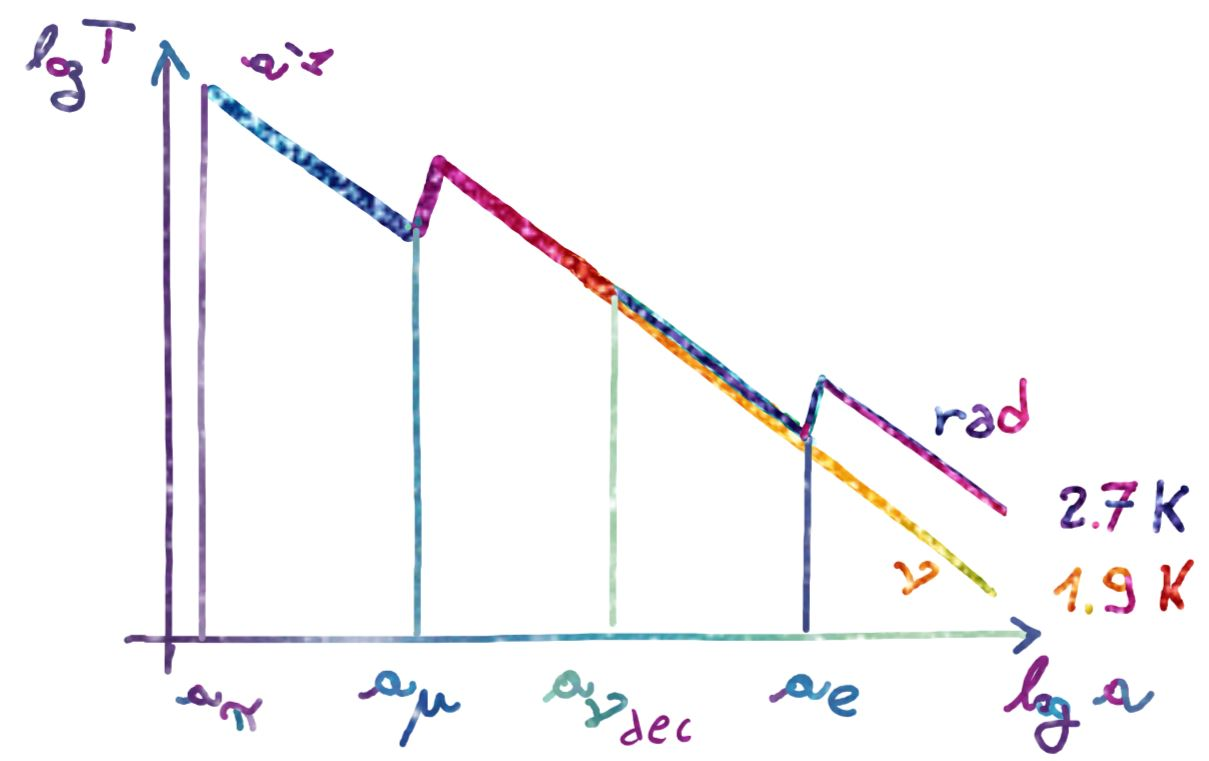
\includegraphics[width=.7 \textwidth]{Pictures/5/annichilazioni.jpg}
    \caption{Temperatura dal variare di $a$ in seguito a: decadimento del pione $a_\pi$, annichilazione dei muoni $a_\mu$, disaccoppiamento dei neutrini $a_{\nu_{dec}}$ e annichilazione della coppia elettrone-positrone $a_e$.}\label{fig5:salti}
\end{figure}


La differenza di temperatura tra radiazione e neutrini è mantenuta fino ad oggi:
$$
T_+ = T_- \left(\frac{11}{4} \right)^{1/3}\simeq 1.4 ~T_-
$$

La temperatura del neutrino oggi deve quindi essere:
$$
T_{\nu\, 0} \simeq \frac{T_{r\, 0}}{1.4} \simeq 1.9 \, \mathrm{K}
$$

Se il neutrino non ha massa (modello standard delle particelle), vale la relazione $\rho_\nu c^2 =\sigma T^4$, da cui si ottiene un contributo $\Omega_{\nu\, 0}\simeq 0.7 \Omegaro$ da aggiungere alla componente relativistica. 

Se il neutrino avesse massa $10$ eV (numero non a caso), si de-relativizzerebbe a $T\approx T_{eq,\, rad}$. In questo caso $T$ è una pseudo-temperatura, ma vale comunque la relazione $n_\nu \propto T_\nu^3$, che restituisce $n_\nu = 320$ cm$^{-3}$ (cfr. $n_\gamma=420$ cm$^{-3}$). Questa quantità contribuisce in questo caso alla componente di materia oscura. In particolare, assumendo che tutta la materia oscura sia dovuta ai neutrini, si può trovare un limite superiore alla loro massa media (tra i tre tipi):
$$
\left \langle m_\nu \right \rangle \le \frac{\Omegamo ~\rho_{cr}}{n_\nu} \qquad \rightarrow\qquad \left \langle m_\nu \right \rangle \le 10\, \mathrm{eV}
$$

In realtà si sa che il neutrino non ha le propietà che ci piacciono per rappresentare tutta la materia oscura (è troppo ``caldo'') e come si vedrà dovrà essere minore di qualche decimo di eV. 


\section{Nucleosintesi Primordiale}
I fenomeni che caratterizzano la nucleosintesi erano già studiati negli anni `40 in associazione con gli interni stellari e le bombe atomiche. È considerata una delle prove fondamentali a favore del modello del Big Bang perché riesce a spiegare molto bene le abbondanze degli elementi leggeri (ciò che le stelline del Prof. Ferraro non possono spiegare). In particolare può giustificare l'alta abbondanza di elio $Y=0.25$. Le condizioni cosmologiche impediscono la formazione di elementi più pesanti a causa delle elevatissime temperature, il problema sarà la formazione del deuterio (che è un collo di bottiglia). Inoltre il modello ha predetto l'esistenza di un fondo cosmico a $T=5$ K, scoperto 30 anni dopo. 

\vspace{1em}
\noindent Le assunzioni del modello standard della nucleosintesi primordiale sono:


\begin{table}[ht]
    \def\arraystretch{1.5}
    \begin{tabular}{lll}

    \textbf{1)} & $T\ge 10^{12}$ K $\quad$  (\textit{hot Big Bang}) \\
    \textbf{2)} & General Relativity $+$ Fisica delle Particelle \\
    \textbf{3)} & Universo sufficientemente Omogeneo e Isotropo  \\
    \textbf{4)} & Cinque o meno tipologie di neutrini \\
    \textbf{5)} & Neutrini non degeneri \\
    \textbf{6)} & Non esistono troppe regioni di antimateria \\
    \textbf{7)} & $\vec{B}$ trascurabili  \\
    \textbf{8)} & Non esistono particelle esotiche \\
    \end{tabular}
    \end{table}

Le condizioni di base sono (1), (2) e (3), in particolare la (3) è verificata con l'inflazione (paradigma non presente nei primi modelli di nucleosintesi). Le condizioni (4), (5) e (8) sono aggiunte a posteriori per evitare la sovrapproduzione di He. La condizione (6) è necessaria per evitare la sovrapproduzione di energia, mentre la (7) viene adottata per non complicare troppo i modelli.  

\subsection{Formazione del deuterio}
Questa è la fase più critica per via dell'alta probabilità del deuterio di essere fotodissociato. Come si è visto nell'equazione (\ref{eq:nn-vs-np}) vale la relazione $n_n / n_P = \exp{(-1.5\cdot 10^{10}/T)}$. L'equilibrio è mantenuto, mediante i neutrini, dalle reazioni:
$$
n + \nu_e \leftrightharpoons p + e^- \qquad n+e^+ \leftrightharpoons p + {\overbar{\nu}_e}
$$

Inoltre si ha:
$$
x_n \equiv \frac{n_n}{n_{tot}} = \frac{n_n}{n_n + n_p} \simeq 0.17
$$

I neutroni rappresentano il 17\% del totale delle particelle finché l'equilibrio tra neutroni e protoni è mantenuto. In realtà anche dopo il disaccoppiamento dei neutrini ($T_{D\nu}\approx 10^{10}$ K) vi sono reazioni residue che garantiscono $x_n (0)=0.17$ fino a $t_N=20$ s ($T_N=1.3 \cdot 10^{9}$ K). Dopo questo tempo dominerà il processo di decadimento del neutrone $ n \rightarrow p + e^- + {\overbar{\nu}_e}$ con un $\tau_n \approx 900$ s, ossia si avrà:
\begin{equation*}
    x_n = x_n (0)~ e^{(t-t_N) / \tau_n}\simeq 0.17 ~e^{(t-20)/ 900}
\end{equation*}

 Per la produzione del deuterio deve avvenire la reazione: $n+p \leftrightharpoons D + \gamma$ molto sfavorita dalla fotodissociazione. Si parte dall'equaizone di Boltzmann (\ref{eq:boltzmann}), ma in questa fase $\mu\neq 0$ perché non ci sono più antiparticelle. Rispettando le regole di ingaggio che seguono e considerando che $g_D=3$ e $(m_n+m_p-m_D)c^2=2.2$ MeV, si ottiene:
\begin{equation*}
    \mu_n + \mu_p = \mu_D +  (\mu_\gamma =0) \quad \rightarrow \quad x_D=x_n ~x_p \exp{\left(-29.33+\frac{25.82}{T_9} -\frac{3}{2}\ln T_9 - \ln (\Omegab h^2) \right)} 
\end{equation*}
che relaziona la quantità di deuterio in funzione della quantità di $n$ e $p$; in particolare:
\begin{equation}x_D \approx \left\{
    \def\arraystretch{1.5}
        \begin{array}{ll}
            0 & T_9 \gg 1 \\ 
            x_n ~x_p & T_9 = 0.9 \quad\mathrm{per}\quad \Omegab \simeq 10^{-2}
    \end{array}\right. \label{eq:xdeuterio}
\end{equation}

Il deuterio inizierà ad essere significativo quando la temperatura $T_9=0.9$ ($T_9=T\cdot 10^{9}$ K), ossia è tanto alta da contrastare il fattore numerico $-29.33$ e questo avviene a $t^*=200$ s. Nelkj caso in cui $\Omegab \simeq 1$ si avrebbe $T_9=0.9$ a $t^*=300$ s.

\subsection{Formazione dell'elio}
A partire da circa 200 secondi (4 minuti) dopo il Big Bang c'è sufficiente deuterio affinchè - istantaneamente - abbiano inizio le reazioni di produzione dell'elio:
$$
D + D \leftrightharpoons {^3He} + n \qquad {^3He} + D \leftrightharpoons {^4He} + p 
$$
L'abbondanza in massa dell'elio vale:
\begin{equation}
    Y = \frac{m_{He}}{m_{tot}} = 4 \frac{1}{2} \frac{n_n}{n_{tot}} = 2 x_n(t^*)
\end{equation}
Utilizzando le relazioni e $t^*$ trovati in precedenza:
$$
Y\simeq 0.25
$$
Valore che soltanto in parte ($\sim 1/6$) può essere prodotto dagli interni stellari; questo è stato il successo del modello della nucleosintesi. Inoltre si può notare che questo valore dipende poco da $n_{tot}$ perché dominano le interazioni elettrodeboli e non quelle tra nucleoni, motivo per cui funziona con diversi modelli cosmologici ($\Omegab$). È la temperatura che trigghera la formazione dell'elio. 

Le densità dell'univiverso erano tali da non permettere ulteriori reazioni (${^8Be}$, {$^{12}C$), si forma soltanto un po' di $^7{Li}$. 

In conclusione, l'${^4He}$ è praticamente costante al variare di $\Omegab$ con un piccolo trend di crescita dovuto al fatto che più si hanno barioni, prima parte la produzione del deuterio e la produzione di ${^4He}$ è più efficiente. L'abbondanza del deuterio, al contrario, è estrememente sensibile: varia di $8$ dex, variando $\Omegab$ di $3$ dex. Il ${^7Li}$ ha una curva più complessa all'aumentare di $\Omegab$: nel primo regime viene prevalentemente prodotto (${^4He}+{^4He}$), poi viene prevalentemente distrutto (${^7Li}+p\rightarrow 2{^4He}$), infine ri-domina la reazione di produzione ${^7Be+e^- \rightarrow {^7Li}}$.

Dall'osservazione di differenti oggetti, meglio non soltanto locali, si può stimare l'abbondanza media di elementi leggeri nell'universo. Rimane complesso estendere le misure fatte localmente, per questo si hanno grossi errori, ma sono comunque sufficienti da individuare una regione di compatibilità dei dati:
$$
0.01 \le \Omegabo \le 0.15
$$
Questi valori si conoscevano già negli anni `70 e assieme alla misurazione della piattezza dell'universo, si aveva già un'altra evidenza di materia oscura. 

\begin{figure}[ht]
    \centering
    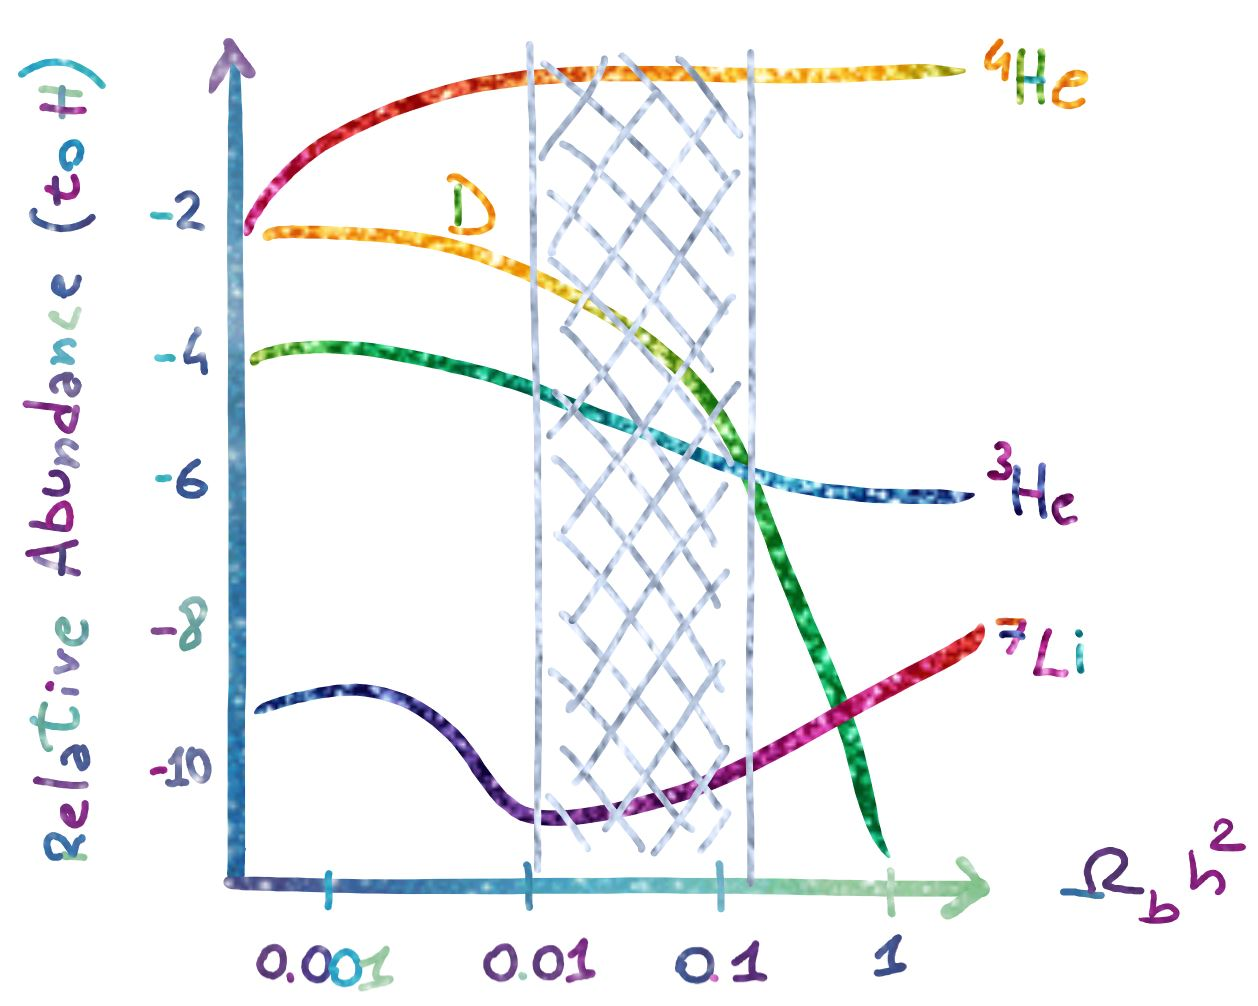
\includegraphics[width=.67\textwidth]{Pictures/5/eleggeriomegab.jpg}
    \caption{Abbondanza relativaall'idrogeno degli elementi leggeri al variare di $\Omegab$. La regione evidenziata corrisponde alle evidenze osservative.}
\end{figure}

\section{Epoca del plasma}
La temperatura diminuisce da $\sim 10^9$ K a $\sim 10^4$ K e l'universo diventa gradualmente più neutro. La successiva re-ionizzazione avverrà solamente per fenomeni di galaxy evolution. Essendo $z_{eq}\sim 1000$, la neutralizzazione formale avviene a $T \sim 2.7\cdot 10^3 $ K.
 In particolare, le principali reazioni e le temperature a cui si ha il 50/50 sono, in ordine:
\begin{equation*}\left\{
    \def\arraystretch{1.5}
        \begin{array}{lll}
        He^{2+}+e^- \leftrightharpoons He^+ + \gamma & 10^4\; \mathrm{K} & \\
        He^+ + e^- \leftrightharpoons He + \gamma &  7\cdot 10^3\; \mathrm{K} & neutralizzazione/\stkout[1pt]{ri}combinazione\; He\\
        H^+ + e^- \leftrightharpoons H + \gamma &  4\cdot 10^3\; \mathrm{K} & neutralizzazione/\stkout[1pt]{ri}combinazione\; H
    \end{array}\right.
\end{equation*}

Prima di questo momento si parla di \textit{epoca del plasma}. 
In una prima fase si hanno: fotoni, $e^-$ e $ p^+$, l'elio (25\% in massa, 6\% in particelle) viene di solito trascurato. Le scale tipiche su cui avvengono le interazioni tra queste componenti sono:

$$ \lambda_D =  \left( \frac{k_BT}{4\pi n_e e^2}\right)^{1/2} \quad \gg \quad \lambda_e \propto n_e^{-1/3} \propto \left ( \frac{m_P}{\rho_{\mathrm{cr},0}\Omegabo}\right)^{1/3} \frac{T_0}{T}$$
Ossia, dentro la sfera di Debye (entro la quale avvengono le interazioni $e^-$ e $p^+$) si ha un gran numero di ioni e quindi un \textit{buon} plasma. Inoltre confrontando il tempo tipico di collisioni tra ioni (attraversamento della sfera di Debye) con il tempo tipico di scattering tra $e^-$ e fotoni (gli $e^-$ perdono momento):
$$ \tau_e = \frac{\lambda_D}{c} \quad \ll \quad \tau_{e\gamma '}=\frac{3m_e}{4\sigma c \rho_r} $$
Per cui non si hanno fenomeni collettivi e $e^-$ e $p^+$ possono considerarsi `accoppiati'. Infine si può verificare che il tempo che serve per mantenerli in equilibrio termico:
$$ \tau_{e^- p^+} = 10^6 (\Omegabo h^2)^{-1} T^{-3/2}\; \textrm{s}  \quad \ll \quad \tau_{exp}$$

Pertanto: elettroni e protoni hanno la stessa temperatura, lo scattering Compton garantisce l'equilibrio con la radiazione e ci si aspetta che questa sia distribuita come un corpo nero.

Le condizioni cambiano quando l'idrogeno \stkout[1pt]{ri}combina.

\subsubsection{Equazioni di Saha}
L'energia di legame dell'idrogeno è $B_H=13.6$ eV corrispondente a una temperatura di $1.6\cdot 10^5$ K. Quando l'universo raggiunge questa temperatura, la temperatura cala ulteriormente rispetto a quanto dettato dal raffreddamento adiabatico. 

Il momento della \stkout[1pt]{ri}combinaizone si fissa quando la frazione di ionizzazione $x=n_e/n_{tot}=0.5$. Elettroni, protoni e idrogeno neutro hanno distribuzione di boltzmann non relativistica (Eq. \ref{eq:boltzmann} sostituendo, per l'$H$, il peso statistico $2$ con $4$). Sapendo che $\mu_p + \mu_e = \mu_H$ e assumendo l'universo elettricamente neutro ($n_e=n_p$):
\begin{equation}
    \frac{n_e n_p}{n_{tot}n_H}=\frac{x^2}{1-x}
\end{equation}
Applicando le distribuzioni di Boltzmann e approssimando $m_p=m_H$:
\begin{equation}
    \frac{x^2}{1-x} = \frac{1}{n_{tot}}\left( \frac{k_B T m_e}{2 \pi \hslash }\right) e^{- B_H / k_B T } 
\end{equation}
Il coefficiente tra parentesi non trascurabile sposta il taglio esponenziale a una temperatura minore di $1.6\cdot 10^5$ K. Inoltre dentro $n_{tot}$ si cela $\Omegabo=0.046^{+0.1}_{-0.01}$, ma in questo caso è la $T$ che comanda. 

\vspace{1em}
La \textbf{ricombinazione} (= prima combinazione) dell'idrogeno avviene quindi a: $$T_{rec,H} \simeq 4000\; \textrm{K} \qquad z_{rec,H}\simeq 1400 \div 1600\quad (1500) $$
Si ricorda che in questo momento si ha 50\% idrogeno neutro e 50\% idrogeno ionizzato, che crollerà esponenzialmente al diminuire di $T$ (stando a questa formula oggi dovrebbe essere $0$, ma non è così per galaxy evolution).
In realtà questa reazione di neutralizzazione non avviene sempre in condizioni di equilibrio (ossia a $\tau_{rec} \sim x/\dt{x} \ll \tau_{exp}$): queste sono già violate a $z\approx 2000$. Svolgendo i conti in condizioni di non equilibrio termico si può verificare che anche a $z\approx few \cdot 100$ c'è una piccola frazione di idrogeno ionizzato, importante per garantire l'accoppiamento materia-radiazione (non spiegabile con solo scattering tra fotoni e idrogeno neutro).

Il vero disaccoppiamento tra le temperature di materia e radiazione è quindi:
$$ z_{dec} \simeq 300 $$

Quando la maggioranza dei fotoni non è più scatterata ed è quindi libera di giungere fino a noi, si osserva la CMB.


La probabilità che un fotone venga scatterato da un elettrone a un certo redshift è:
\begin{equation}
    \mathrm{d}P=-\frac{\mathrm{d}N_\gamma}{N_\gamma}=-\frac{\mathrm{d}I}{I}=\frac{\mathrm{d}t}{\tau_{\gamma e}}=-\d{\tau} \qquad\quad \tau=\int_0^z \frac{xc\rho_m \sigma_T }{m_P}\frac{\d{t}}{\d{z'}}\d{z'}
\end{equation}
Da cui la probabilità che un fotone venga scatterato per l'ultima volta ad un dato redshift è:
\begin{equation}
    -\frac{\d{}}{\d{z}}\left( 1-e^{-\tau} \right)=e^{-\int \tau (z)\d{\tau}}
\end{equation}
Questa probabilità ha una distribuzione gaussiana centrata a $z\simeq 1100$ (detto \textbf{reshift dell'ultimo scattering} con una $FWHM=400$. Questo risultato dipende poco dalla cosmologia. A questi redshift la distribuzione dei fotoni consente di tracciare anche la distribuzione della materia, mentre a redshift maggiori non è possibile ottenere informazioni dalla radiazione.

\newpage
Si hanno quindi tre valori del redshift legati allo stesso fenomeno (ricombinazione dell'idrogeno $z\approx 1000$), ma formalmente diversi:
\begin{example}[Ricombinazione: $\mathbf{z_{rec}=1500}$]
Momento in cui $x=0.5 $
\end{example}
\begin{example}[Disaccoppiamento:  $\mathbf{z_{dec}=300}$]
Momento in cui $T_m=T_r \rightarrow T_m \neq T_r $
\end{example}
\begin{example}[Last Scattering:  $\mathbf{z_{LS}=1100}$]
Picco della distribuzione di probabilità di last scattering.
\end{example}

\vspace{1em}
La conservazione del numero di fotoni $n_\gamma \propto (e^{h\nu /kT}-1)^{-1}$ in un universo in espansione fa sì che la radiazione rimanga distribuita come un corpo nero $I(t_i, \nu)\propto \nu^3 (e^{h\nu /kT}-1)^{-1}$, ma shiftato a frequenze minori, quindi con una $T=T_0(1+z)$. Questo, che è il più bel corpo nero visto in natura è stato osservato dal satellite COBE nel 1991. Una piccola deviazione si verifica a causa dei fotoni generati dalla ricombinazione, ma questo si vede solo nelle code e non nel picco dove $n_\gamma$ è altissimo. Ulteriori deviazioni dal corpo nero possono essere legate a fenomeni di fisica primordiale. In particolare a quelli avvenuti a $10^7 < z < 10^4 $, quando la CMB non sarebbe stata in grado di riportarsi all'equilibrio (a $z$ ancora più alto la termalizzazione è rapidissima, mentre a $z$ ancora più basso il tempo si dilata può termalizzare con calma). Queste vengono dette \textit{anisotropie primarie} e vanno anch'esse cercate nelle code della plankiana. Tra le \textit{anisotropie secondarie} vi è l'effetto Sunyaev–Zeldovich (coming soon...). Con questo si chiude la prima metà del corso, siamo a metà, coraggio!
